\section{Introdução}

% Bluetooth Overview
Bluetooth é uma tecnologia de comunicação sem fio de curto alcance desenvolvida
pelo BLuetooth Special Interest Group, também conhecido como Bluetooth SIG. Esta
tecnologia está presente em uma vasta gama de dispositivos, sendo utilizada em
smartphones, computadores, automóveis, tablets entre
outros.\cite{gomez2012overview}

O Bluetooth Low Energy, ou BLE, é uma das formas de operação previstas na
especificação da versão 4.0 do Bluetooth. Junto com o BLE, o documento também
especifica a operação do tipo Basic Rate, também chamado de BR, dando
continuidade as formas de operação definidas nas versões anteriores do
bluetooth.\cite{ble4core}
Um dispositivo bluetooth pode operar na forma Single Mode, sendo compatível
apenas com BLE, ou na forma Dual Mode, sendo compatível com as duas
formas de operação. \cite{ble4core}

% O que o BLE faz para ser Low Power

\subsection{Formas de operação} %GAP
As formas de operação do BLE são definidas pelo General Access Profile,
abreviado como GAP, e este perfil determina que um dispositivo possui 4 formas
de operação: Broadcaster, Observer, Slave e Central. \cite{ble4core}

Como Broadcaster, o dispositivo opera somente como transmissor de dados,
enviando pacotes de dados periodicamente, ação denominada Advertising, que
podem conter informações sobre o dispositivo e indicam a presença de um 
dispositivo num dado local. Quando um dispositivo opera apenas como
broadcaster, ele não está aberto a receber conexões.\cite{ble4core}

Como Observer, o dispositivo opera somente como um receptor de dados, recebendo
apenas os pacotes de advertising enviados por outros dispositivos
BLE.\cite{ble4core}

Como Peripheral, o dispositivo suporta estabelecer uma conexão como slave. Para
outro dispositivo detectar sua presença e iniciar uma conexão, é necessário que
o peripheral opere antes como um broadcaster, indicando sua
presença.\cite{ble4core}

Como Central, o dispositivo suporta múltiplas conexões como master e é sempre o
responsável por iniciar as conexões com um peripheral. Para detectar um
peripheral, é necessário que a central opere como um observer para detectar a
presença de outros dispositivos.\cite{ble4core}. Um dispositivo é capaz de
suportar múltiplas formas de operação ao mesmo tempo.\cite{ble4core}

\subsection{Meio físico}
% Descrição do meio físico
O BLE opera na frequência de 2.4GHz utilizando 40 canais de 2MHz com
frequências de centro de 2402MHz a 2480MHz. Existem dois tipos de transmissão: a
transmissão de dados, que é feita em 37 dos canais disponíveis com a capacidade
de transmissão de 1Mbit/s, que é realizada pelos dispositivos operando como
central ou como peripeheral; e o Advertising, que é feito nos outros 3 canais
restantes com as frequências de 2402MHz, 2426MHz e 2480MHz, que
é realizado nos dispositivos operando como broadcaster.\cite{ble4core}

A tabela \ref{tab:adv_channel_list} mapeia os canais de rádiofrequência para os canais
utilizados pelo BLE com suas respectivas identificações e finalidades. 	

\begin{center}
	\centering 
	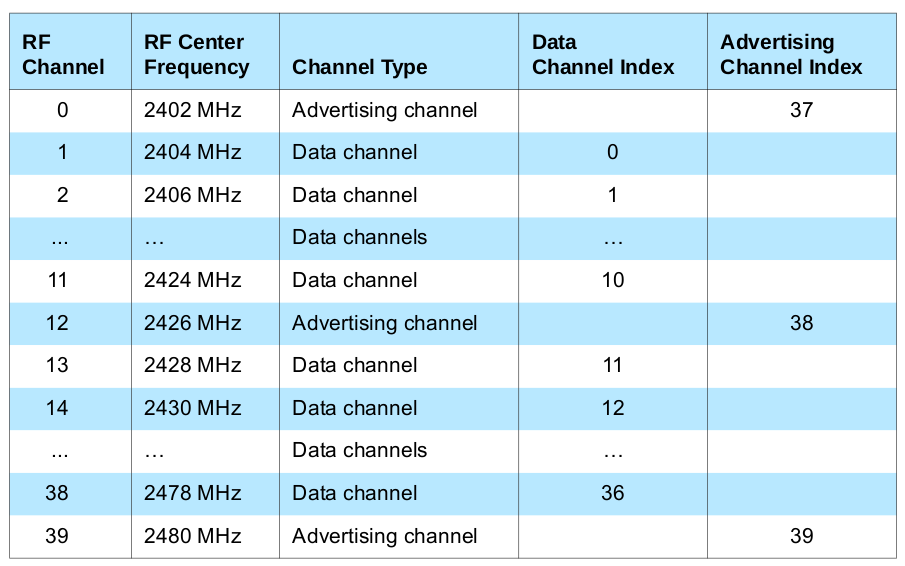
\includegraphics[width=0.8\linewidth]{adv_ch_map.png}
	\captionof{table}{Mapeamento dos canais de RF para os canais do BLE \cite{ble4core}}
	\label{tab:adv_channel_list}
\end{center} 
 
\subsection{Advertising}
Advertising é a ação de transmitir pacotes de dados de forma pública para todos
os dispositivos capazes de recebê-los nos três canais de advertising, com a
finalidade principal de indicar a presença do dispositivo no local e é
realizada pelos dispositivos que operam como periperal ou como broadcaster. O
advertising também indica se o dispositivo é conectável ou não.
Logo após o envio de um pacote de advertising em um canal, o broadcaster fica 
apto a receber uma mensagem por um instante, e quando um peripheral ou central
recebem um advertising, podem ser solicitadas mais  informações nesse mesmo 
instante através da transmissão de um pacote de Scanner  Request que é enviado,
e quando o broadcaster recebe esta solicitação um pacote  chamado Scan Response
é enviado.\cite{ble4core} 

Durante este instante em que o broadcaster pode receber uma solicitação, é
possível também que uma central faça uma solicitação de início de conexão,
portanto, uma conexão só pode ser iniciada no envio de um pacote de advertising.
\cite{ble4core}

\subsection{Identificação dos dispositivos}
\label{subsection:id}
No BLE os dispositivos são identificados através do Device Address, ou Endereço
do Dispositivo, que possui 48 bits. O endereço do dispositivo também é chamado
de MAC Address, ou Media Access Control Address. Existem dois tipos de endereço:
o endereço público e o aleatório.\cite{ble4core}

O endereço público é um endereço controlado pela IEEE Registration Authority e
deve seguir o padrão IEEE 802-2001. Um endereço público é composto por 24 bits
definidos que identificam uma empresa, chamado de Company ID, sendo estes os
bits mais significativos. Os 24 bits menos significativos são atribuídos a
critério da própria empresa. Este endereço não é alterado ao longo da vida do
dispositivo.\cite{ble4core}

O endereço aleatório pode ser transmitido ou não e possui tipos: o estático e o
privado. O endereço aleatório estático é um endereço que não muda ao longo de um
ciclo de operação do dispositivo, porém pode ser alterado após o dispositivo
reiniciar, e possui apenas 3 regras para ser definido: os dois bits mais
significativos devem ser 1, os bits restantes não podem ser todos 0, os bits
restantes não podem ser todos 1. \cite{ble4core}

Já o endereço aleatório privado pode ser solucionável ou não. Quando um endereço
é solucionável há uma chave compartilhada entre os dispositivos BLE utilizada
para decodificar o endereço, e é necessário que os dois bits mais significativos
sejam 0 e 1, respectivamente. Quando o endereço é não solucionável, a formação é
similar ao endereço estático, porém os dois bits mais significativos devem ser
0 e o dispositivo pode mudar este endereço a qualquer momento de sua
operação. \cite{ble4core}

\subsection{Aplicações BLE}

As aplicações BLE, também chamadas de BLE Profile, são disponibilizadas quando
os dispositivos estão conectados. A estrutura de uma aplicação é composta pelos
serviços e características usadas.

Uma aplicação é composta por um ou mais serviços. Um serviço é um conjunto de
valores associados para cumprir uma funcionalidade específica de um dispositivo.
Cada um dos valores associados num serviço é chamado de caracterísca, que além
do valor possui informações sobre este valor. A figura \ref{fig:ble_profile}
mostra como a aplicação é estruturada.

\begin{center}
	\centering 
	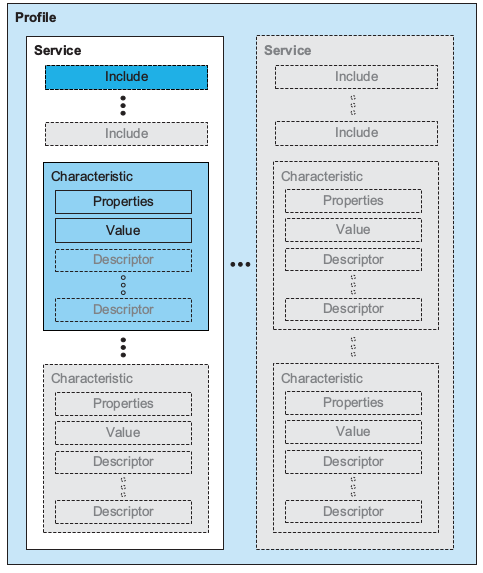
\includegraphics[width=0.6\linewidth]{ble-profile.png}  
	\captionof{figure}{Estrutura de uma aplicação BLE \cite{ble4core}}
	\label{fig:ble_profile}
\end{center}  

Cada serviço é identificado por um Universal Unique Identifier, ou UUID.
Serviços que são definidos e padronizados pelo Bluetooth SIG possuem um UUID de
16 bits. Há também a possibilidade de criar serviços customizados que possuem um
UUID de 128 bits.

Cada característica também possui um UUID de 16 ou 128 bits. Além da
indentificação e dos valores, as características possuem uma série de
propriedades. São elas:

\begin{itemize}[noitemsep]
  \item \textbf{Read}: indica que uma característica pode ser lida.
  \item \textbf{Write Without Response}: indica que uma característica pode ser
  escrita, porém não há uma resposta a escrita.
  \item \textbf{Write}: indica que uma característica pode ser escrita com
  resposta ao término do procedimento
  \item \textbf{Notify}: indica que o valor da característica será enviado sem
  solicitação e sem confirmação de entrega.
  \item \textbf{Indicate}: equivalente ao Notify, porém com confirmação de
  entrega
  \item \textbf{Authenticated Signed Write}: a escrita só é permitida após a
  autenticação do dispositivo
\end{itemize}

\subsection{Pacotes BLE}

Os pacotes transmitidos no ar pelo BLE seguem o formato definido na figura
\ref{fig:ble_packet}. Normalmente os campos do pacote de advertising são
preenchidos pelo controlador BLE ou pelas bibliotecas de BLE utilizadas num
projeto. Para a aplicação BLE normalmente se tem acesso a uma Application
Programming Interface, ou API, para se definir os formatos e as informações
contidas no pacote.

\begin{center}
	\centering 
	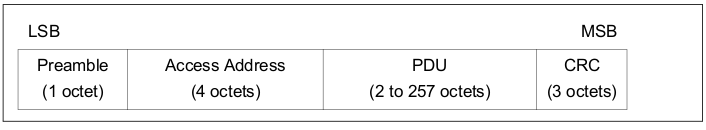
\includegraphics[width=0.9\linewidth]{ble-packet.png}  
	\captionof{figure}{Estrutura de um pacote BLE \cite{ble4core}}
	\label{fig:ble_packet}
\end{center}  

O campo PDU, ou Packet Data Unit, é o campo em que ficam armazenados os dados
para transmissão, e pode ser formatado de duas formas: Advertising Channel PDU e
Data Channel PDU.

O Data Channel PDU é utilizado durante a conexão BLE, e nele são trocados as
informações dos serviços, características e os parâmetros de conexão e possui um
conjunto de mensagens definidos no volume 6, seção 2.4 da especificação do
bluetooth. \cite{ble4core}.

O Advertising Channel PDU é utilizado durante o Advertising, possui a estrutura
mostrada na figura \ref{fig:adv_pdu}. O campo Header possuindo a estrutura
mostrada na figura \ref{fig:adv_header}, e é referente ao cabeçalho do pacote
de advertising.

\begin{center}
	\centering 
	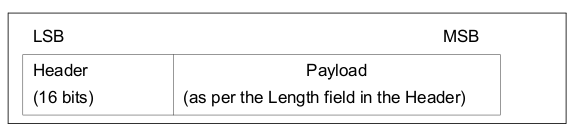
\includegraphics[width=0.9\linewidth]{ble-adv-pdu.png}  
	\captionof{figure}{Estrutura de um pacote de Advertising \cite{ble4core}}
	\label{fig:adv_pdu}
\end{center}  

\begin{center}
	\centering 
	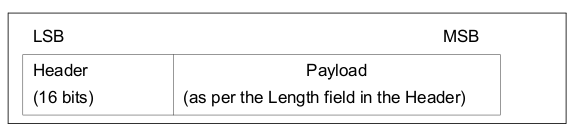
\includegraphics[width=0.9\linewidth]{ble-adv-pdu.png}  
	\captionof{figure}{Cabeçalho de um pacote de Advertising \cite{ble4core}}
	\label{fig:adv_header}
\end{center}  

A tabela \ref{tab:pdu_type} define o significado dos valores que podem ser
preenchidos no campo PDU Type.

\begin{center}
	\centering 
	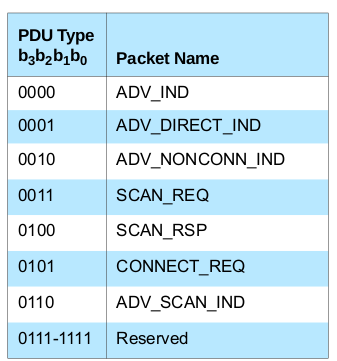
\includegraphics[width=0.5\linewidth]{ble-adv-header-values.png}  
	\captionof{table}{Valores possíveis para o cabeçalho do Advertising
	\cite{ble4core}}
	\label{tab:pdu_type}
\end{center}  

Cada valor para o cabeçalho indica um padrão de advertising:

\begin{itemize}[noitemsep]
  \item \textbf{ADV\_ IND}: dispositivo conectável por qualquer central
  \item \textbf{ADV\_DIRECT\_IND}: dispositivo conectável apenas para
  dispositivos específicos
  \item \textbf{ADV\_NONCONN\_IND}: dispositivo não conectável
  \item \textbf{SCAN\_REQ}: solicitação de um pacote de Scan Request
  \item \textbf{SCAN\_RSP}: envio de pacote de Scan Response
  \item \textbf{CONNECT\_REQ}: solicitação de início de conexão
  %\item \textbf{ADV_SCAN\_IND}: solicitação de início de conexão
\end{itemize} 

A figura \ref{fig:adv_payload} mostra como é o formato do campo payload do
pacote de advertising. O campo AdvA contém o endereço de 48 bits do dispositivo,
descrito na seção \ref{subsection:id}.
\begin{center}
	\centering 
	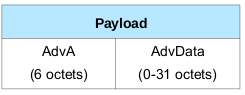
\includegraphics[width=0.4\linewidth]{ble-adv-payload.png}  
	\captionof{figure}{Formato do campo Payload \cite{ble4core}}
	\label{fig:adv_payload}
\end{center}  

A figura \ref{fig:advdata_format} define como devem ser organizados os dados
dentro do campo AdvData, que possui um limite de 31 bytes.
\begin{center}
	\centering 
	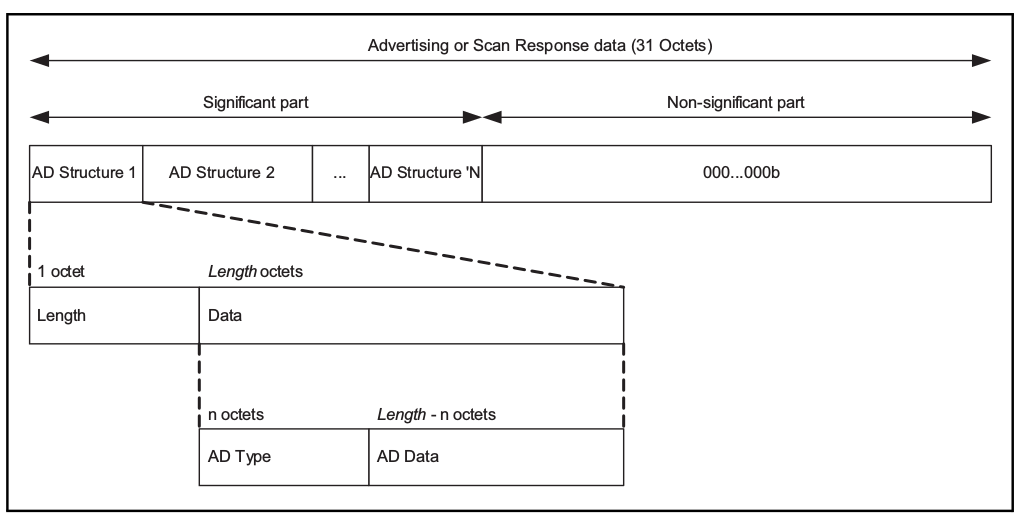
\includegraphics[width=\linewidth]{adv-payload.png}  
	\captionof{figure}{Estrutura do AdvData \cite{ble4core}}
	\label{fig:advdata_format}
\end{center} 

A especificação suplementar do bluetooth em conjunto com a página Bluetooth
Assigned Numbers especifica quais são os formatos para o campo AD Data e quais
são os AD Types possíveis. \cite{ble4sup} \cite{GAPDataTypes}
